% 
% topic Template for ME3050 -  Dynamics Modeling and Controls - Tennessee Technological University
%
% Spring 2020 - Summer 2020
% Tristan Hill, May 07, 2020
% Dyanmics Review - Topic 1 - What is System Dynamics?
%

\documentclass{beamer}                         % for presentation (has nav buttons at bottom)
%\documentclass[handout]{beamer}  % for handout 
\usepackage{beamerthemesplit}
\usepackage{amsmath}
\usepackage{listings}
\usepackage{multicol}

\beamertemplateballitem

\definecolor{TTUpurple}{rgb}{0.3098, 0.1607, 0.5176} % TTU Purple (primary)
\definecolor{TTUgold}{rgb}{1.0000, 0.8666, 0.0000} % TTU Gold (primary)

\setbeamercolor{palette primary}{bg=TTUpurple,fg=TTUgold}
\setbeamercolor{palette secondary}{bg=black,fg=TTUgold}
\setbeamercolor{palette tertiary}{bg=black,fg=TTUpurple}
\setbeamercolor{palette quaternary}{bg=TTUgold,fg=black}
\setbeamercolor{structure}{fg=TTUpurple} % itemize, enumerate, etc
\setbeamercolor{section in toc}{fg=TTUpurple} % TOC sections

%\usefonttheme{professionalfonts}

\newcommand{\Lagr}{\mathcal{L}} % lagrangian

\newcommand{\vspccc}{\vspace{6mm}\\} % large vertical space
\newcommand{\vspcc}{\vspace{4mm}\\}   % medium vertical space
\newcommand{\vspc}{\vspace{2mm}\\}     % small vertical space

\newcommand{\hspcccc}{\hspace{10mm}} % large horizontal space
\newcommand{\hspccc}{\hspace{6mm}} % large horizontal space
\newcommand{\hspcc}{\hspace{4mm}}   % medium horizontal space
\newcommand{\hspc}{\hspace{2mm}}     % small horizontal space


\author{ME3050 - Dynamics Modeling and Controls} % original formatting from Mike Renfro, September 21, 2004

\newcommand{\TNUM}{1\hspace{2mm}} % topic Number 
\newcommand{\topictitle}{What is System Dynamics?} % first line of title (used by beamer)
\newcommand{\sectiontitle}{Dynamics Review }% second line of the title of this presentation (used by TWH)

\title{\sectiontitle - \topictitle}

\date{May 29, 2020}

\begin{document}

\lstset{language=MATLAB,basicstyle=\ttfamily\small,showstringspaces=false}

\frame{\titlepage \center\textbf{Topic \TNUM - \topictitle}\vspace{5mm}\\}

% Section 0: Outline


\frame{

\large \textbf{Topic \TNUM - \topictitle} \vspace{3mm}\\

%Topics : \vspace{3mm}\\ % ' topics' are beamer 'sections' - TWH

\begin{itemize}
	\item Welcome Back!\vspace{3mm}\\ % Section 1
	\item Definition of {\it Dynamics}\vspace{3mm}\\% Section 2
	\item Modeling and Analysis \vspace{3mm}\\ %Section 3
	\item Model Based Design\vspace{3mm}\\ % Section 4
	%\item Example\vspace{3mm}\\ % Section 5 - 5 is almost too many...
\end{itemize}
}

% Section 1
\section{Welcome Back!}

\frame{
\frametitle{Welcome to New Video topics}
\large{\it Welcome Back!\vspace{3mm}\\}

\begin{itemize}
\item Things are going to be different but we will still learn! \vspace{3mm}\\
\item These new outlines should help keep me/us on track.  \vspace{3mm}\\
\item The material will be organized in $\sim 10$ min videos, and you can watch them at anytime. \vspace{3mm}\\
\end{itemize}

}

% Section 2
\section{Definition of Dynamics}

\frame{
\frametitle{Definition of Dynamics}

\large
Dynamics is ...\vspcc

the study of how moving objects behave, \vspcc
or \vspcc
an area of mechanics that studies movement and its causes,\vspcc
or \vspcc
%\Large{"The dynamical system concept is a mathematical formalization for any fixed "rule" which describes the time dependence of a point's position in its ambient space. "} \vspace{5mm} \\

{\it system dynamics} is the study of {\bf modeling} and {\bf analysis} of dynamical systems as a function of time.\vspc



}

\frame{
\frametitle{Dynamics vs System Dynamics}

\large
Dynamics: find state of \underline{object} at \underline{a specific instant in time} \vspccc

System Dynamics: find state of \underline{system} as a \underline{function of time}  \vspc

$\rightarrow$ Leads to use of differential equations. $m\ddot{x}+c\dot{x}+kx=f(t)$

}

% Section 3
\section{Modeling and Analysis}

\frame{
\frametitle{What is Mathematical Modeling?}

A mathematical model is a description of a system using mathematical concepts and language. The process of developing a mathematical model is termed mathematical {\bf modeling} ... \vspc
...  used in the natural sciences and engineering disciplines ...  \href{https://en.wikipedia.org/wiki/Mathematical_model}{\tiny Wikipedia}

\begin{itemize}
\item Model Simplification
\item Force and Loading Analysis with FBDs
\item Fundamental Laws Lead to Equations of Motion
\item Newton's Second Law and Conservation of Energy

\end{itemize}

}

\frame{
\frametitle{What is Analysis?}

{\bf Analysis} is the process of breaking a complex topic or substance into smaller parts in order to gain a better understanding of it... \href{https://en.wikipedia.org/wiki/Analysis}{\tiny Wikipedia}

\begin{itemize}
\item Study Model to find  of System Response
\item Time-Domain analysis: examine system response in time to various inputs and initial conditions
\item Frequency-Domain analysis: examine system response when subject to sinusoidal inputs


\end{itemize}

}

% Section 4
\section{Model Based Design}

\frame{
\frametitle{Model Based Design}

Model-Based Design (MBD) is a mathematical and visual method of addressing problems associated with designing complex control, signal processing and communication systems. It is used in many motion control, industrial equipment, aerospace, and automotive applications... \href{https://en.wikipedia.org/wiki/Model-based_design}{\tiny Wikipedia}

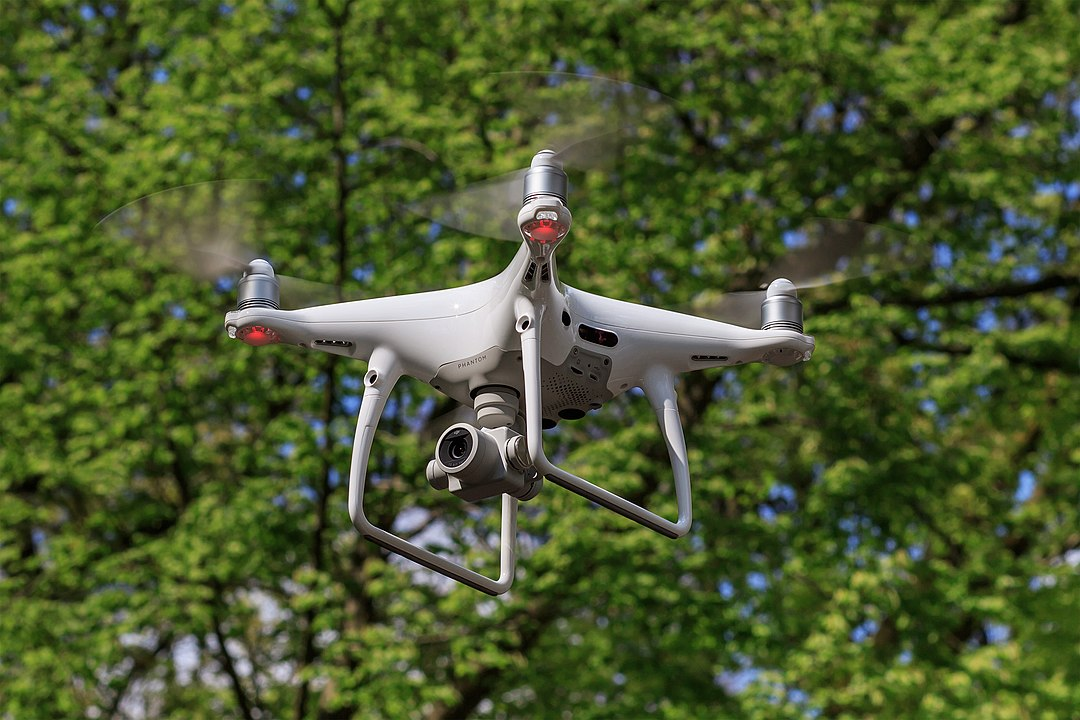
\includegraphics[scale=.08]{dji_phantom_fig2.jpg}\hspccc
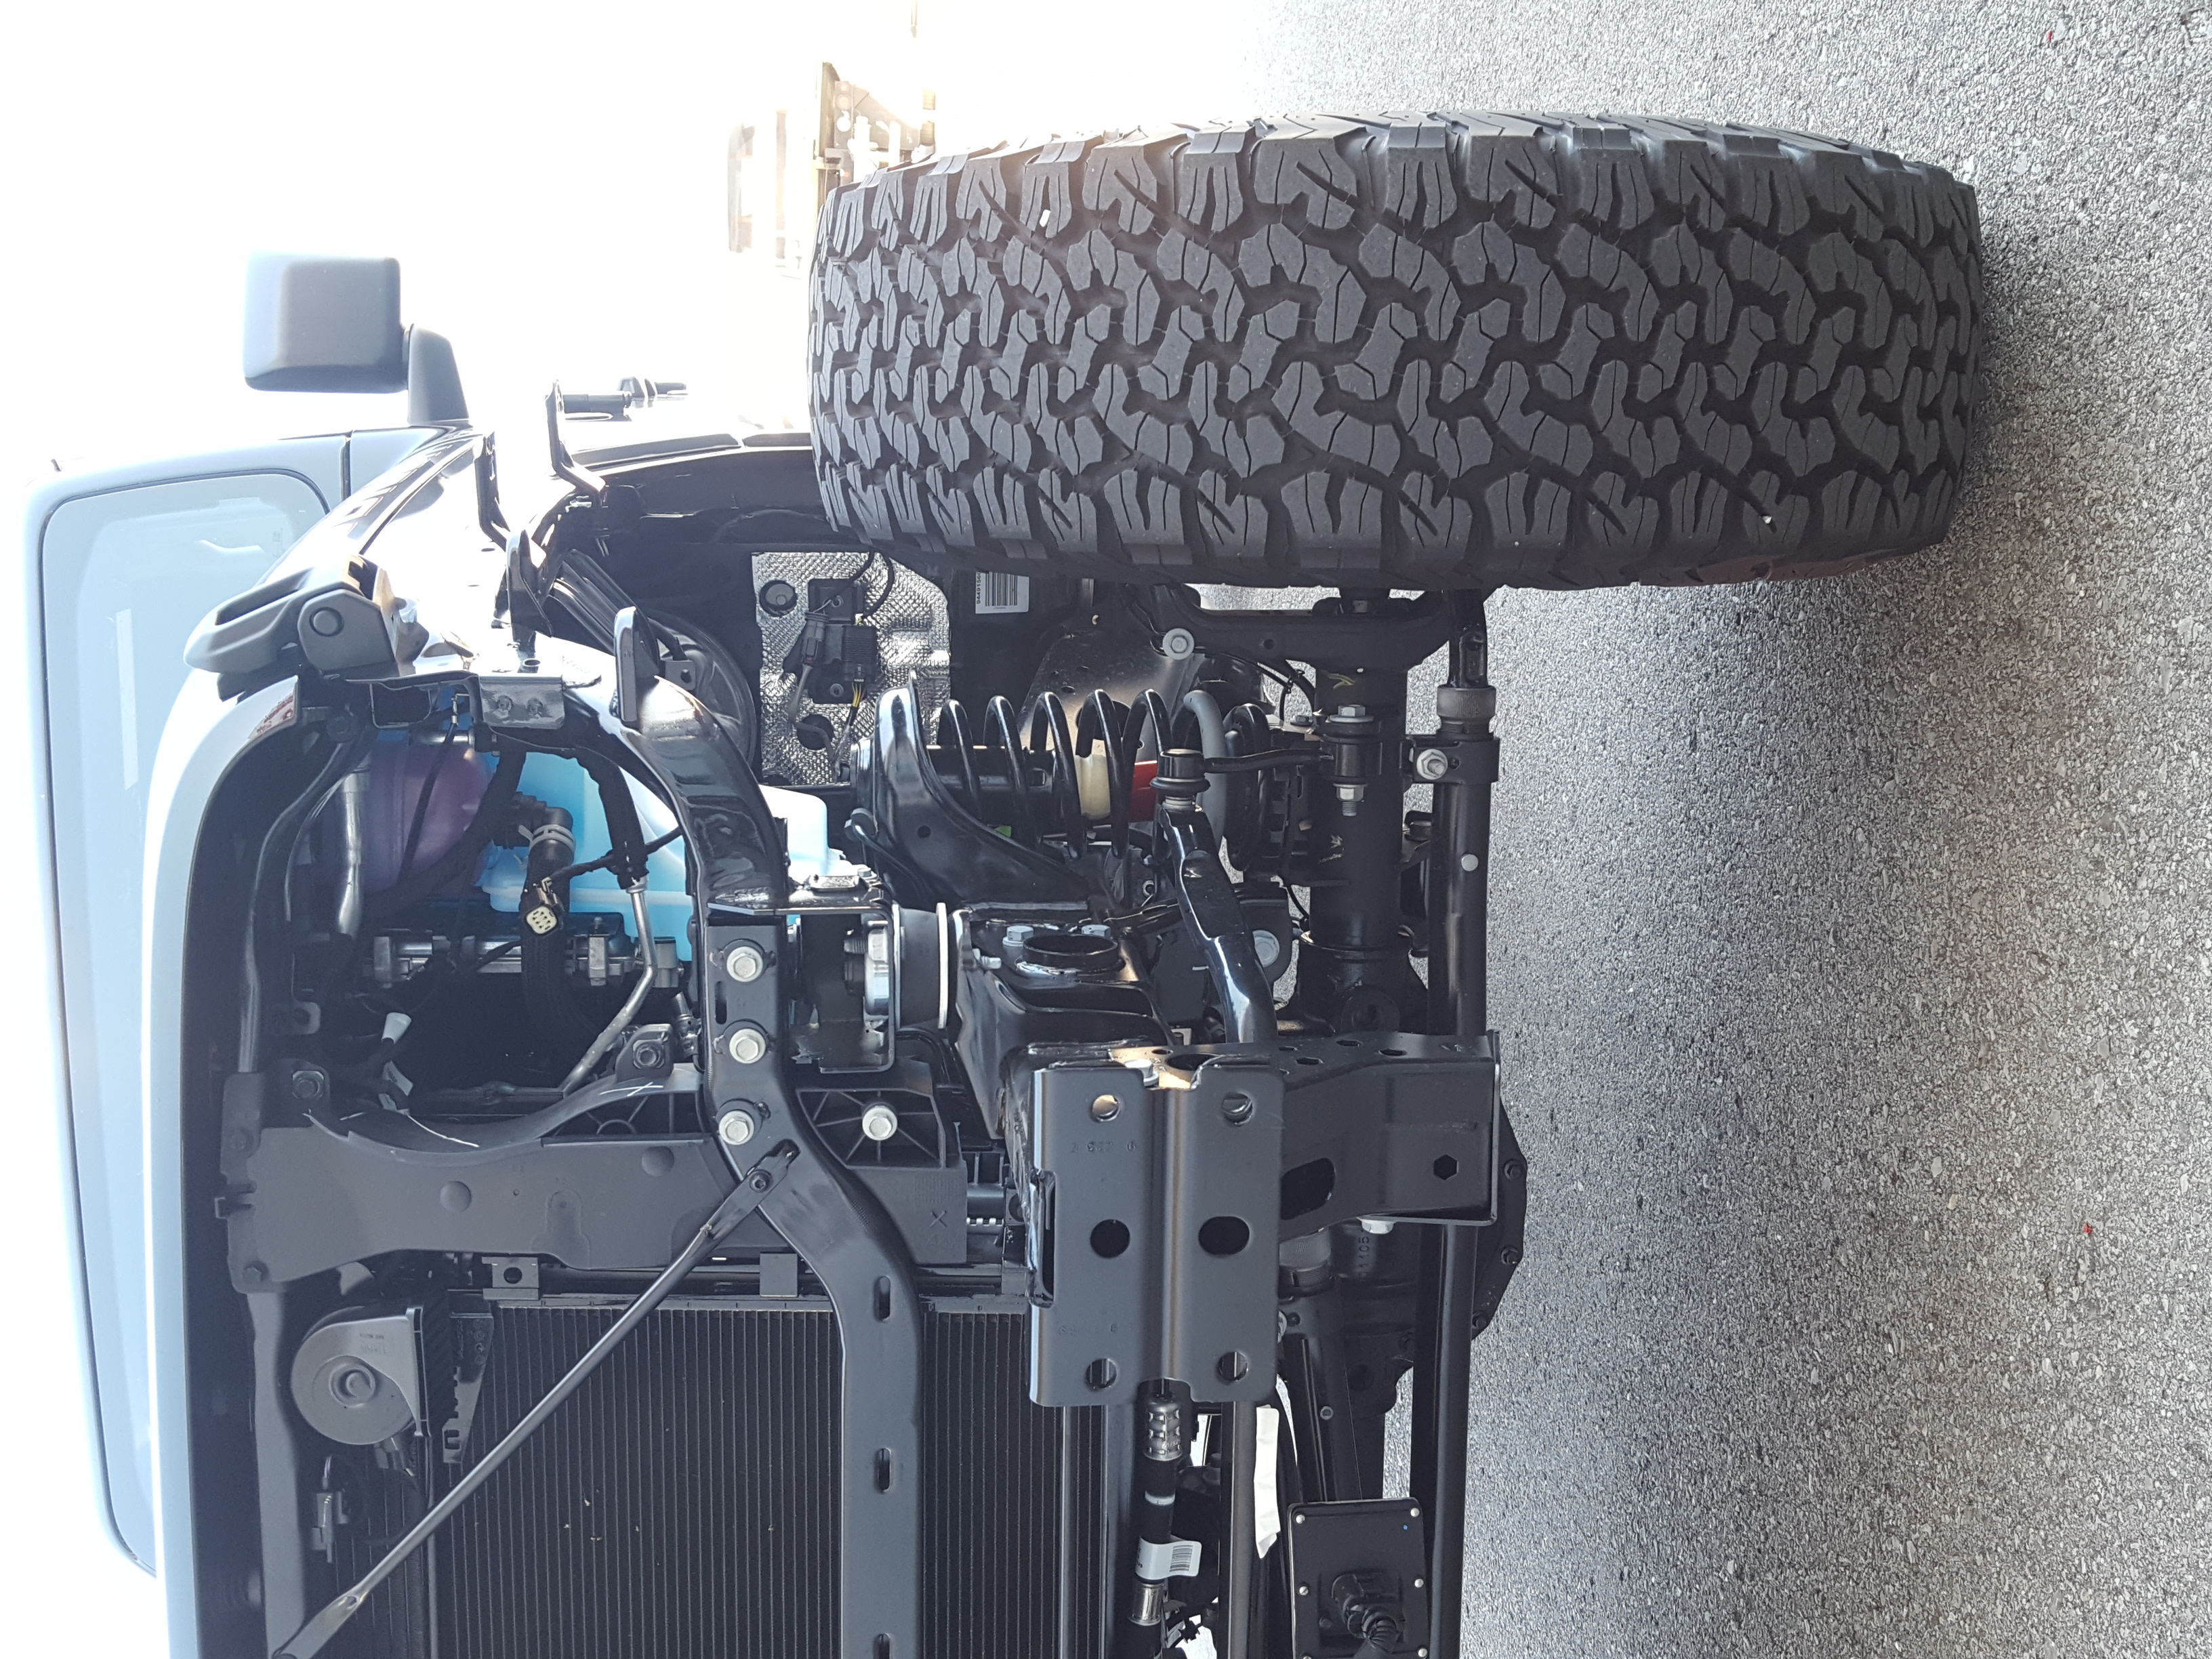
\includegraphics[scale=.025,angle=-90,origin=c]{jeep_01.jpg} \hspccc
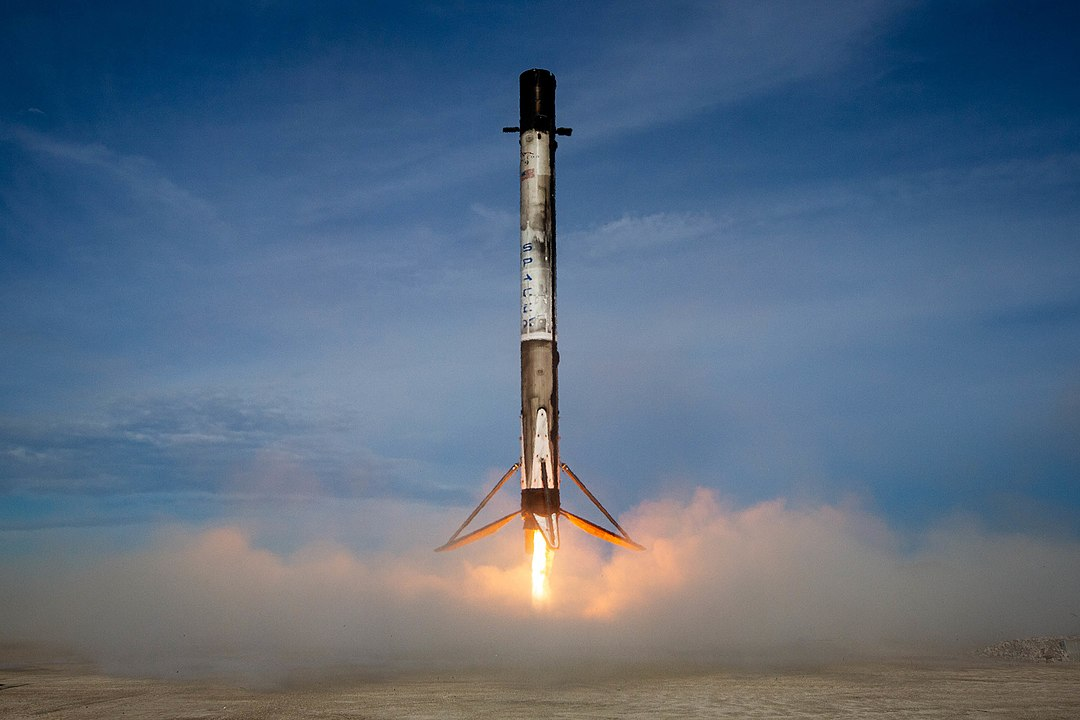
\includegraphics[scale=.1]{falcon9_fig2.jpg} \\
{\tiny\href{https://en.wikipedia.org/wiki/Phantom_(UAV)}{Image: Wikipedia} \hspace{20mm}Image: TH \hspace{20mm}\href{https://en.wikipedia.org/wiki/SpaceX\#/media/File:CRS-18_Mission_(48380511427).jpg}{Image: Wikipedia} }
}

\end{document}





